% Source of ../final_jumping_ring.pdf, the report shown on projects/jumping-ring.html.
% Rebuild:  python analysis.py && latexmk -pdf report.tex && cp report.pdf ../final_jumping_ring.pdf
\documentclass[11pt]{article}
\usepackage[T1]{fontenc}
\usepackage{lmodern}
\usepackage[margin=1in]{geometry}
\usepackage{amsmath}
\usepackage{graphicx}
\usepackage{booktabs}
\usepackage{float}
\usepackage{caption}
\usepackage{subcaption}
\usepackage{xcolor}
\usepackage{listings}
\usepackage{microtype}
\usepackage[hidelinks]{hyperref}
\hypersetup{pdftitle={Jumping-Ring Dynamics: How Temperature Tunes the Thomson Coil Launch}, pdfauthor={Songgun Lee}}

\newcommand{\tC}[1]{$#1\,^{\circ}\mathrm{C}$}
\setlength{\parskip}{0.5em}
\setlength{\parindent}{0pt}
\captionsetup{font=small, labelfont=bf}
\lstset{language=Python, basicstyle=\ttfamily\scriptsize, columns=fullflexible, keepspaces=true,
  showstringspaces=false, breaklines=true, frame=single, rulecolor=\color{black!25},
  commentstyle=\color{black!55}\itshape, keywordstyle=\bfseries}

\title{Jumping-Ring Dynamics: How Temperature Tunes the Thomson Coil Launch}
\author{Songgun Lee}
\date{PHYS 20CL final project, UC Santa Barbara, June 2025\\[2pt]
{\small Revised November 2026; see the note at the end}}

\begin{document}
\maketitle

\begin{abstract}
\noindent
I explored how ring temperature alters the upward force generated in the classic ``jumping-ring''
(Thomson coil) experiment. Using a copper solenoid powered by a 120~V AC line and an aluminum ring
(diameter 6.2~cm, height 1.2~cm, thickness 0.8~cm), I measured peak jump heights at four
temperatures: \tC{-196} (liquid N$_2$), \tC{-52.3} (freezer), \tC{22.4} (room) and \tC{148} (hot
plate). A FLIR ONE thermal camera read the ring temperature before launch at the three warmer
settings, while a DJI Osmo Pocket~3 captured 60~fps side-view video. Heights were extracted with
FIJI from meter-stick reference frames and corrected for the 17.9~cm coil elevation. Averaging five
trials per temperature, a straight-line fit to the three camera-measured temperatures gives
$H = (-0.232 \pm 0.011)\,T + (71.83 \pm 1.65)$~cm, a 5\,\% relative uncertainty on the slope: the
colder the ring, the higher it jumps. The liquid-nitrogen point, $98.8 \pm 2.4$~cm, lies 18.6~cm
below the extrapolated line, so a straight line describes the data only over the \tC{200} span between \tC{-52} and \tC{148}. The results are consistent with a model in which decreased resistivity, and
thus larger induced current, at low temperature enlarges the magnetic impulse.
\end{abstract}

\section*{Introduction}

Electromagnetic launchers fascinate because they turn invisible fields into dramatic motion. In the
Thomson jumping-ring demonstration a 60~Hz current in a vertical solenoid induces eddy currents in a
conductive ring; Lenz's law then repels the ring upward. Textbooks treat the impulse
semi-quantitatively by assuming the ring behaves as a perfect shorted turn whose inductance and
resistance remain constant. Resistance, however, is highly temperature dependent for metals,
dropping by a factor of $\approx 10$ from \tC{150} down to liquid-nitrogen temperatures. Lower
resistance should increase both the peak induced current $I_\mathrm{ring} = \mathcal{E}/R(T)$ and
the magnetic flux linkage, thereby boosting launch speed and apex height. Surprisingly, the
temperature lever is rarely explored in undergraduate laboratories.

Here I systematically varied ring temperature from \tC{148} down to \tC{-196} and measured the corresponding
jump height. My goal was twofold: (i) quantify the $H(T)$ relationship and (ii) test whether a
simple linear model suffices over this broad range. A by-product is a clear, student-friendly
dataset illustrating the practical impact of resistivity versus temperature.

\section*{Methods}

\subsection*{Apparatus}

The launcher is a coil of 65 turns of copper wire on an iron core. The coil is 12.9~cm tall, and the
ring rests 17.9~cm above the floor before launch. The aluminum ring has a diameter of 6.2~cm, a
thickness of 0.8~cm and a height of 1.2~cm (Figure~\ref{fig:apparatus}).

\begin{figure}[H]
\centering
\begin{subfigure}{0.3\textwidth}\centering
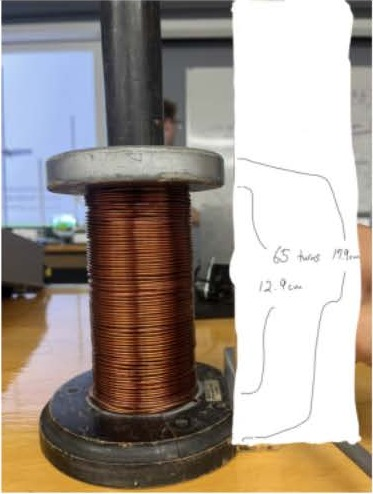
\includegraphics[height=5.2cm]{fig/coil.jpg}\caption{}\end{subfigure}
\begin{subfigure}{0.4\textwidth}\centering
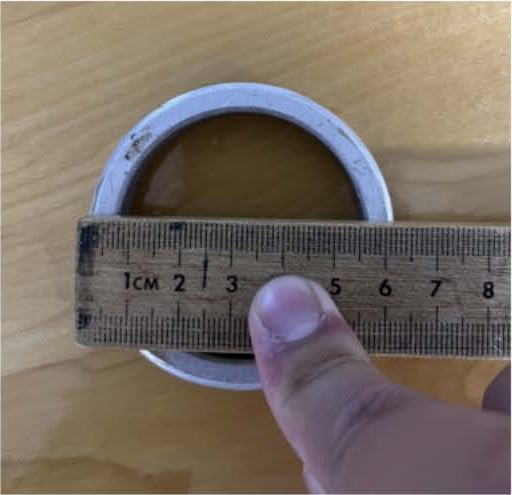
\includegraphics[height=5.2cm]{fig/ring_ruler.jpg}\caption{}\end{subfigure}
\caption{(a) The coil. The handwritten labels read 65 turns, 12.9~cm and 17.9~cm. (b) The ring.}
\label{fig:apparatus}
\end{figure}

\subsection*{Temperature control}

\emph{Cryogenic:} The ring is submerged in liquid nitrogen for 3 minutes inside a cup, then launched
within 4~s to minimise warm-up. \emph{Freezer:} I put the ring inside a freezer that goes to
\tC{-80} for 1 hour, but the ring reached \tC{-52.3}. \emph{Room:} Ambient \tC{22.4} serves as
baseline. \emph{Hot:} I used a heating plate to heat my ring. The ring reached just under \tC{150},
then launched within 4~s to minimise cool-down.

For the freezer, room, and hot-controlled ring, I used FLIR ONE, an apparatus attaching to iPhone to
measure temperature. However, the FLIR ONE had limits from \tC{-60} to \tC{150} and the cryogenic
ring clearly went to temperatures below \tC{-60}, so its temperature was not measured. I take it to
be the boiling point of nitrogen, \tC{-196}, plot that point separately and leave it out of the
fit. For the hot ring, I made sure that it was above \tC{148} and below \tC{150}; I use \tC{148} in
the analysis.

Figure~\ref{fig:flir} shows how even the temperature was across the ring: right after it was taken
out of the freezer, and right off the hot plate.

\begin{figure}[H]
\centering
\begin{subfigure}{0.3\textwidth}\centering
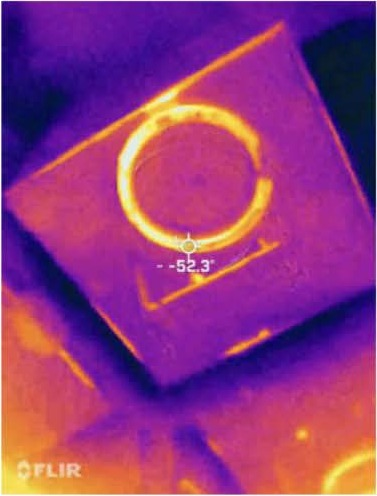
\includegraphics[height=5.2cm]{fig/flir_freezer.jpg}\caption{}\end{subfigure}
\begin{subfigure}{0.3\textwidth}\centering
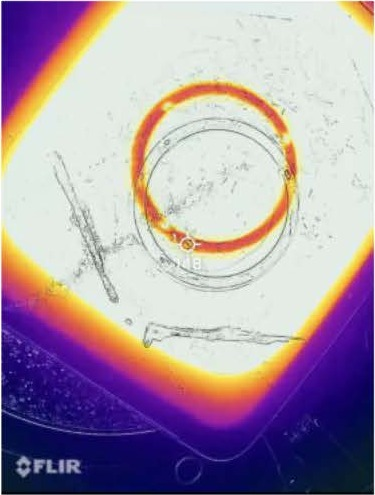
\includegraphics[height=5.2cm]{fig/flir_hotplate.jpg}\caption{}\end{subfigure}
\caption{Thermal images of the ring (a) just out of the freezer, reading \tC{-52.3}, and (b) just
off the hot plate.}
\label{fig:flir}
\end{figure}

\subsection*{Motion capture}

A DJI Osmo Pocket~3 records 3K60 video. I used frame-by-frame analysis using Adobe Premiere Pro to
catch the exact moment the ring reached its maximum height, and used FIJI to measure the height.
However, there were mistakes made in the cryogenic measurement, as the ring exceeded one meter, and
the camera was not placed exactly at eye-level of the ring's highest point, thus creating over a
20\,\% uncertainty. Figure~\ref{fig:capture}(a) shows an example of the mistake,
Figure~\ref{fig:capture}(b) shows how I was able to bring the camera to eye-level of the jumping
ring, and Figure~\ref{fig:capture}(c) shows how I used FIJI to measure the height reached.

In the example of Figure~\ref{fig:capture}(c), the temperature was \tC{22.4} and the scale was
4.125~pixels/mm. Then, I estimated the ``center of the ring'' to the closest 10~cm unit, which was
90~cm. The length was $(900 - 15.193)$~mm, which gave around 88.5~cm.

\begin{figure}[H]
\centering
\begin{subfigure}{0.22\textwidth}\centering
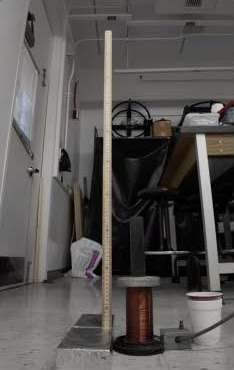
\includegraphics[height=4.6cm]{fig/camera_low.jpg}\caption{}\end{subfigure}
\begin{subfigure}{0.34\textwidth}\centering
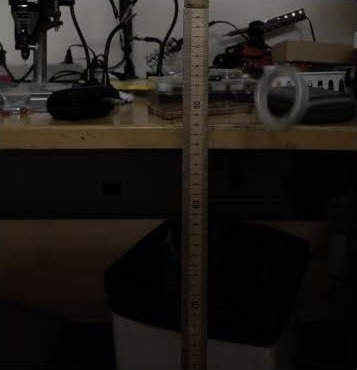
\includegraphics[height=4.6cm]{fig/camera_level.jpg}\caption{}\end{subfigure}
\begin{subfigure}{0.36\textwidth}\centering
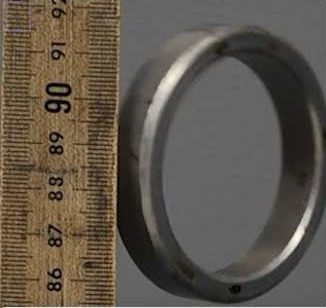
\includegraphics[height=4.6cm]{fig/fiji.jpg}\caption{}\end{subfigure}
\caption{(a) Camera too low. (b) Camera level with the top of the jump. (c) Measuring the height in
FIJI against the meter stick; FIJI reported a length of 15.193~mm.}
\label{fig:capture}
\end{figure}

\section*{Results}

Table~\ref{tab:data} gives the mean net jump height at each temperature. The analysis code, which
contains every raw height, follows.

\begin{table}[H]
\centering
\begin{tabular}{rcc}
\toprule
Ring temperature $T$ & Mean net height $H$ (cm) & Standard deviation $s$ of 5 trials (cm) \\
\midrule
\tC{-196} (not measured) & 98.80 & 2.38 \\
\tC{-52.3} & 81.36 & 3.01 \\
\tC{22.4} & 68.66 & 2.10 \\
\tC{148} & 37.46 & 0.09 \\
\bottomrule
\end{tabular}
\caption{Net height is the height above the floor minus the 17.9~cm starting height of the ring.}
\label{tab:data}
\end{table}

\lstinputlisting[lastline=75]{analysis.py}

\begin{verbatim}
Slope     m = -0.232 +/- 0.011  cm / C
Intercept b = 71.83 +/- 1.65 cm
\end{verbatim}

\begin{figure}[H]
\centering
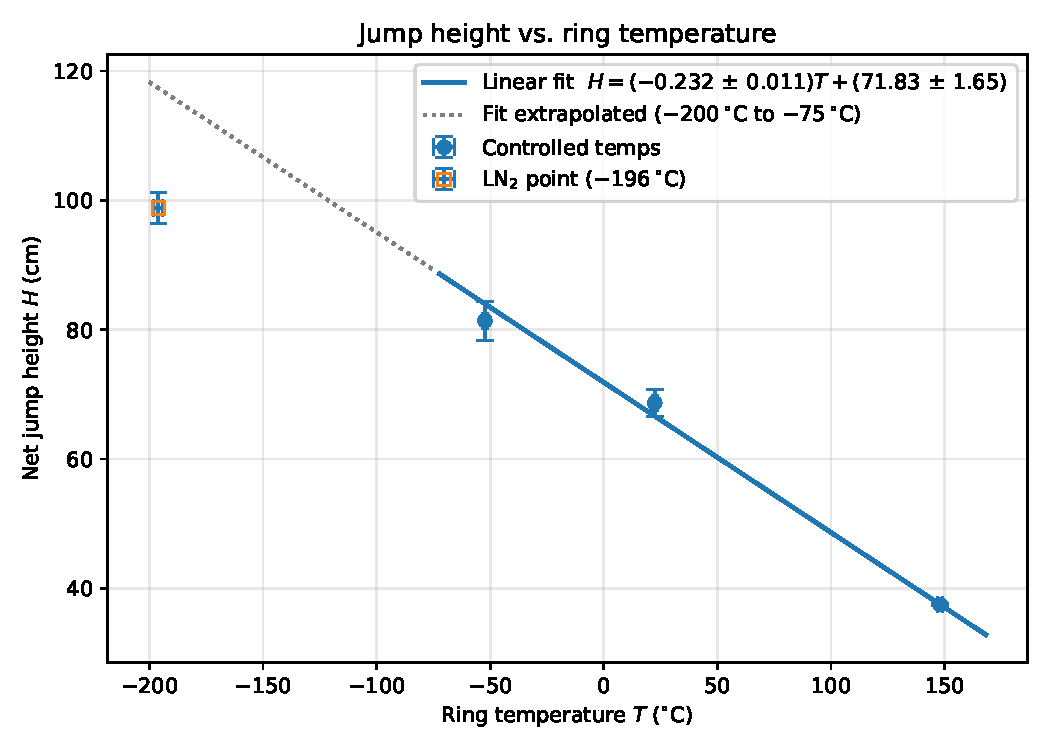
\includegraphics[width=0.74\textwidth]{fit.pdf}
\caption{Net jump height against ring temperature. The line is fitted to the three filled points
only. Vertical error bars are the standard deviation of the five trials.}
\label{fig:fit}
\end{figure}

The fit uses the three temperatures measured with the thermal camera. It gives a slope of
$-0.232 \pm 0.011$~cm/$^{\circ}$C and an intercept of $71.83 \pm 1.65$~cm, with $\chi^2 = 1.7$ for
one degree of freedom.

The liquid-nitrogen point is plotted but not fitted. The extrapolated line predicts 117.4~cm at
\tC{-196}; the measured height is $98.8 \pm 2.4$~cm, which is 18.6~cm lower. Read the other way,
the fitted line reaches 98.8~cm at about \tC{-116}. Either the ring had warmed well above \tC{-196}
by the time it launched, or its height was misread because of the camera angle, or the linear trend
does not continue down to liquid-nitrogen temperature. This experiment cannot tell these apart.

\subsection*{Uncertainty analysis}

To translate pixel measurements in FIJI to physical distances, I calibrated each frame with the
wooden ruler: a 10~cm segment on the ruler was set equal to the corresponding pixel length, giving a
conversion factor of about 44~px\,cm$^{-1}$ in the high-resolution (3K at 60~fps, portrait) videos
(41~px\,cm$^{-1}$ in the example frame above) and $11.5 \pm 0.5$~px\,cm$^{-1}$ in the earlier
landscape clips. The dominant systematic (scaling) error comes from the 1~px cursor placement
uncertainty:
\[
\sigma_\mathrm{scale} =
\begin{cases}
\pm 0.023~\mathrm{cm} & \text{(high-resolution)}\\
\pm 0.087~\mathrm{cm} & \text{(low-resolution)}
\end{cases}
\]
I adopt the more conservative $\pm 0.09$~cm for all heights. The camera timing is negligible: at
60~fps the frame nearest the apex is at most half a frame (8~ms) away from it, and because the
ring's vertical velocity at the apex is $\approx 0$, this changes the height by less than
0.05~cm, well below $\sigma_\mathrm{scale}$. The ring-centre selection (the ring may tilt or
translate in the frame) adds another $\pm 0.10$~cm; combining this in quadrature with
$\sigma_\mathrm{scale}$ gives a total single-measurement height uncertainty
\[
\sigma_H = \sqrt{0.09^2 + 0.10^2} \approx \pm 0.13~\mathrm{cm}.
\]

For each temperature I recorded five trials. The sample standard deviation $s$ of the five heights
is 3.0~cm (freezer), 2.1~cm (room), 0.09~cm (hot ring) and 2.4~cm (LN$_2$). Except for the hot
ring, this trial-to-trial spread is much larger than $\sigma_H$, so it dominates. I use $s$ as the
uncertainty of each mean height, both for the error bars and as the weight in the fit. This is
larger than the standard error of the mean, $s/\sqrt{N}$ with $N = 5$. For the hot ring, where four
of the five readings were identical, $s$ is smaller than $\sigma_H$; adding $\sigma_H$ in
quadrature changes neither the slope nor its uncertainty at the quoted precision.

If each mean is instead weighted by its standard error, $s/\sqrt{N}$ combined in quadrature with
$\sigma_H$, the slope is unchanged, $-0.232 \pm 0.005$~cm/$^{\circ}$C, but $\chi^2$ rises to 8.3
for one degree of freedom. The three means then differ from a straight line by more than their
standard errors allow, so the $\pm 0.011$ quoted above is the more cautious uncertainty.

The error bar drawn on the liquid-nitrogen point is only the spread of its five trials. It does not
include the camera-angle error described under Motion capture.

The temperature error bars are rough estimates: $\pm 1\,^{\circ}$C for the three temperatures read
with the thermal camera, and $\pm 2\,^{\circ}$C drawn on the liquid-nitrogen point, whose
temperature was not measured. They are shown on the plot but are not used in the fit.

\section*{Discussion}

The Thomson jumping-ring experiment demonstrates the interplay between electromagnetic induction,
material properties, and temperature in determining the ring's jump height. The linear relationship
observed, $H = (-0.232 \pm 0.011)\,T + (71.83 \pm 1.65)$~cm, indicates that temperature
significantly affects the ring's behavior. As temperature decreases from \tC{148} to \tC{-52}, the
mean jump height increases from 37.5~cm to 81.4~cm. This trend can be attributed to the temperature
dependence of the ring's resistivity. For aluminum, resistivity decreases at lower temperatures,
dropping by a factor of approximately 10 from \tC{150} to liquid-nitrogen temperatures (\tC{-196}).
According to Ohm's law and Lenz's law, lower resistivity results in a higher induced current,
$I_\mathrm{ring} = \mathcal{E}/R(T)$, where $\mathcal{E}$ is the induced electromotive force and
$R(T)$ is the temperature-dependent resistance. A higher induced current strengthens the opposing
magnetic field generated by the ring, increasing the repulsive force and thus the jump height.
Lenz's law governs the ring's motion by ensuring that the induced current opposes the change in
magnetic flux. When the AC solenoid is energized, the changing magnetic field induces eddy currents
in the conductive ring. These currents create a magnetic field that opposes the solenoid's field,
resulting in a repulsive force that launches the ring upward. The strength of this force depends on
the induced current, which is inversely proportional to the ring's resistance. At \tC{-196}, the
ring's enhanced conductivity (due to reduced resistivity) amplifies the induced current, leading to
a stronger opposing magnetic field and a higher jump.

The ring's shape and material properties also play a critical role. The toroidal geometry (6.2~cm
diameter, 0.8~cm thickness, 1.2~cm height) ensures a uniform current path, maximizing the
efficiency of the induced current in generating a magnetic field. A non-conductive or differently
shaped ring, such as one with a gap, would reduce the current loop's effectiveness, lowering the
jump height.

Temperature uncertainties, as noted in the uncertainty analysis, contribute to variations in the
jump height. The single-measurement uncertainty in height, $\sigma_H \approx 0.13$~cm, is small compared with
the spread between repeated trials (up to 3.0~cm), which dominates. Systematic errors matter most
for the liquid-nitrogen point: the FLIR ONE cannot read below \tC{-60}, so that temperature was not
measured, and the camera angle made its height unreliable. That point is therefore not part of the
fit and does not affect the slope. With three temperatures and two fitted parameters, the fit has
only one degree of freedom, so it is not a strict test of linearity, and with standard-error weights the agreement with a
straight line is marginal. Additionally, the ring's thermal expansion or contraction at
extreme temperatures could alter its dimensions, though this effect is minimal for aluminum over
the given range.

\section*{Conclusion}

This experiment quantified the relationship between temperature and jump height in the Thomson
jumping-ring setup. Between \tC{-52} and \tC{148}, a \tC{200} span, the jump height falls as the ring warms, and a straight line describes it to within the spread
between trials. The liquid-nitrogen point falls below the extrapolated line, so the linear
relation should not be extended to \tC{-196}. The decrease in resistivity at lower temperatures
enhances the ring's conductivity, leading to a stronger induced current and a greater opposing
magnetic field. Consequently, due to Lenz's law, the ring experiences a more significant repulsive
force, propelling it to greater heights as the temperature decreases. Based on the fitted
relationship, if the temperature increases by \tC{1}, the ring is projected to jump approximately
0.232~cm lower because the increased resistivity reduces the induced current, weakening the
magnetic repulsion. These findings underscore the role of temperature in electromagnetic launch
systems and provide a practical demonstration of fundamental physics principles in action.

\section*{Possible future improvements}

Several improvements could enhance the accuracy and scope of this experiment. First, the FLIR ONE's
limited temperature range (\tC{-60} to \tC{150}) introduced uncertainty in the cryogenic
measurements; using a thermal camera or thermocouple with a broader range, such as one capable of
accurately measuring down to \tC{-196}, would provide more precise temperature data. Second, the
camera positioning error during high jumps (e.g., at \tC{-196}) resulted in a 20\,\% uncertainty in
height measurements. Employing a taller setup with multiple synchronized cameras at
different heights could capture the ring's apex more accurately, reducing systematic errors. Third,
the statistical spread in jump heights (0.09 to 3.0~cm) suggests variability in launch conditions;
increasing the number of trials per temperature (e.g., from 5 to 10) and controlling for
environmental factors like air currents could reduce this spread. Finally, exploring a wider range of ring
materials (e.g., copper, silver) or geometries (e.g., varying thickness or introducing a gap) could
provide deeper insights into the interplay between material properties and electromagnetic
induction.

\section*{Things to do differently}

Reflecting on the experimental design, a few adjustments could improve future iterations. First, I
would ensure consistent camera alignment by mounting the DJI Osmo Pocket~3 on a tripod with a
height-adjustable mechanism, allowing precise eye-level positioning for all jump heights,
especially at cryogenic temperatures where the ring exceeded one meter. Second, I would minimize
the time between removing the ring from its temperature environment and launching it (currently
4~s) by streamlining the setup process, as rapid warming or cooling during transfer likely
introduced small temperature variations. Using an insulated transfer mechanism or performing
launches in a controlled temperature chamber could mitigate this issue. Lastly, I would incorporate
real-time temperature monitoring during the jump to capture any dynamic heating effects immediately
after launch, complementing the post-levitation measurement of \tC{32}. These changes would enhance
the precision of the temperature-jump height relationship and provide a more comprehensive
understanding of the system's behavior.

\section*{Supplementary material}

\subsection*{Explanation of Lenz's law and the electromagnetism behind it}

Lenz's law is a fundamental principle in electromagnetism that describes the direction of an
induced electromotive force (EMF) and the resulting current in a conductor when it experiences a
changing magnetic field. Formulated by Heinrich Lenz in 1834, the law states that the induced
current will flow in a direction such that its own magnetic field opposes the change in the
magnetic flux that produced it. This is a direct consequence of the conservation of energy,
ensuring that the system does not generate motion or current without an external driving force.

\subsection*{Electromagnetism behind Lenz's law}

The phenomenon is rooted in Faraday's law of electromagnetic induction, which states that a
changing magnetic field through a conductor induces an EMF, given by
$\mathcal{E} = -\frac{d\Phi_B}{dt}$, where $\Phi_B$ is the magnetic flux. The negative sign in
Faraday's law reflects Lenz's law, indicating that the induced EMF generates a current whose
magnetic field counteracts the original change in flux. Magnetic flux $\Phi_B$ is defined as
$\Phi_B = B \cdot A \cdot \cos\theta$, where $B$ is the magnetic field strength, $A$ is the area of
the conductor loop, and $\theta$ is the angle between the field and the normal to the loop. When
the magnetic field through the conductor changes, due to the motion of a magnet or, as in the
jumping-ring experiment, the alternating current (AC) in a solenoid, this change induces a
circulating current in the conductor. In the context of the Thomson jumping-ring experiment, the
solenoid, powered by a 60~Hz AC source, produces a rapidly oscillating magnetic field. This
changing field penetrates the conductive aluminum ring placed above it, inducing eddy currents
within the ring. According to Lenz's law, these induced currents create their own magnetic field
that opposes the increase in the solenoid's field. The opposing magnetic field results in a
repulsive force between the solenoid and the ring, launching the ring upward. The strength of this
force depends on the magnitude of the induced current, which is governed by Ohm's law,
$I = \mathcal{E}/R$, where $R$ is the ring's resistance. Lower resistance (as occurs at lower
temperatures due to decreased resistivity) increases the current, amplifying the opposing magnetic
field and thus the launch height.

\subsection*{Mechanism in the jumping-ring experiment}

The AC solenoid's alternating current causes the magnetic field to oscillate, inducing eddy
currents in the ring that follow Lenz's law by opposing the field change. This opposition creates a
dynamic repulsive force, lifting the ring. The ring's toroidal shape ensures a closed current path,
enhancing the efficiency of the induced magnetic field. The temperature effect observed in the
experiment, higher jumps at lower temperatures, arises because reduced resistivity increases the
induced current, strengthening the opposing field and the resulting force, consistent with Lenz's
law's predictive framework. In summary, Lenz's law is a key principle that ensures the induced
response in a conductor counteracts the initiating magnetic change, driving the electromagnetic
behavior observed in systems like the jumping ring. This interplay of induced currents and opposing
fields exemplifies the broader principles of electromagnetic induction and energy conservation.

\subsection*{Temperature increase after jumps}

During the course of the jumping-ring experiment, an interesting observation was made regarding the
thermal effects on the ring post-jump. After conducting jumps at room temperature, it was noticed
that the ring exhibited a noticeable increase in temperature compared to its initial state. To
investigate this further, the ring was allowed to levitate by continuously activating the solenoid
with a constant current for one minute. This sustained levitation caused the ring's temperature to rise significantly, as
measured with the FLIR ONE thermal camera, reaching approximately \tC{32} after exactly one minute.
Figure~\ref{fig:levitation}(a) shows the ring in a levitated state while the coil is continuously
energized by pressing the button, demonstrating the electromagnetic force keeping it aloft.
Figure~\ref{fig:levitation}(b), captured using the FLIR ONE, confirms the temperature increase to
\tC{32}, highlighting the heat generated by the induced eddy currents during the prolonged exposure
to the solenoid's magnetic field. This suggests that the energy dissipation from the induced
currents during levitation contributes to a measurable heating effect, providing additional insight
into the thermal behavior of the ring under continuous electromagnetic influence.

\begin{figure}[H]
\centering
\begin{subfigure}{0.3\textwidth}\centering
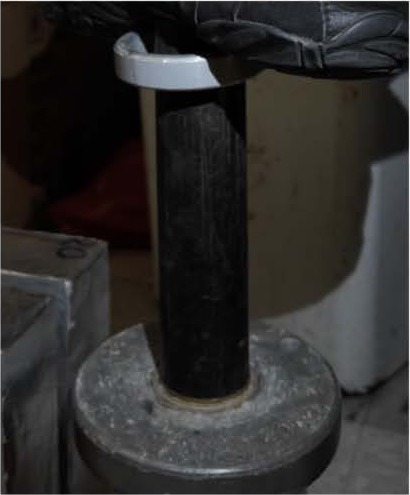
\includegraphics[height=5.2cm]{fig/levitation.jpg}\caption{}\end{subfigure}
\begin{subfigure}{0.3\textwidth}\centering
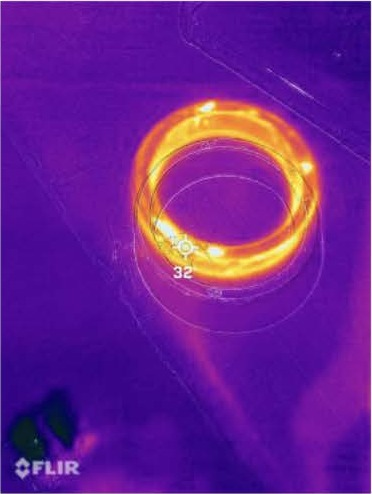
\includegraphics[height=5.2cm]{fig/flir_levitation.jpg}\caption{}\end{subfigure}
\caption{(a) The ring levitating while the coil is energized. (b) Thermal image after one minute of
levitation, reading \tC{32}.}
\label{fig:levitation}
\end{figure}

\section*{Revision note (November 2026)}

The measurements, the analysis code and the fit are those of the report submitted in June 2025.
This revision corrects text that disagreed with them: the abstract quoted a fit,
$H = (0.167 \pm 0.011)\,T + 33.7$~cm, that did not come from the analysis and said the
liquid-nitrogen point lay on the line; the discussion called the aluminum ring copper; and the
uncertainty section misstated the spreads between trials and how the error bars were set. The
figures are the original photographs, and the plot is regenerated from the same code.

\end{document}
